\documentclass[../main.tex]{subfiles}

\begin{document}


\practica{9}{Creación automática de BSP}

    \subsection{Objetivos}
        \begin{itemize}
            \item Aprender a utilizar herramientas avanzadas de desarrollo de sistemas empotrados como STMCubeMX.
            \item Comprender la planificación de pines al utilizar un microcontrolador.
        \end{itemize}

    \subsection{Fundamentos teóricos}
       
        Hasta ahora, hemos estado desarrollando nuestros propios paquetes BSP para trabajar con nuestra placa. Así, hemos conseguido facilitar el uso mediante funciones auxiliares que nos permitan realizar configuraciones o acciones. Para saber exactamente cómo trabajar con la placa, hemos tenido que consultar \REFMAN, \BRDMAN, \DSMAN, \PMMAN, \ANMAN, \dots.

        Normalmente (y así es en el caso de ST, desarrolladora del \MCU), se proporcionan paquetes software que ya contienen toda la funcionalidad preprogramada, para evitarnos tener que hacerlo manualmente. Estos paquetes son desarrollados por los ingenieros de ``software'', basándose en los manuales proporcionados por los ingenieros de ``hardware''.

        En ocasiones, se proporciona un único paquete genérico con toda la funcionalidad, y es responsabilidad del usuario final decidir qué y cómo lo utiliza. Aunque esto tiene la ventaja de empaquetar toda la funcionalidad en un único conjunto de librerías, tiene el inconveniente de agrandar el código al incluir mucha funcionalidad que quizá no utilicemos. En el caso de ST, proporcionan una herramienta para crear un BSP a medida con únicamente los elementos que queramos incluir. Es esta funcionalidad la que vemos a continuación.

    \subsection{Desarrollo de la práctica}

        \subsubsection{Creación del BSP con STMCubeMX}

            Lo primero de todo es abrir la aplicación STMCubeMX (\Cref{fig:cubemx_00_init}). Tenemos varias funciones: 
            \begin{itemize}
                \item Ver los proyectos ya creados.
                \item Empezar un proyecto eligiendo un procesador, una placa, o un ejemplo preparado por ST.
                \item Actualizar la aplicación e incluir paquetes software nuevos.
            \end{itemize}
            
            \begin{figure}
                \centering
                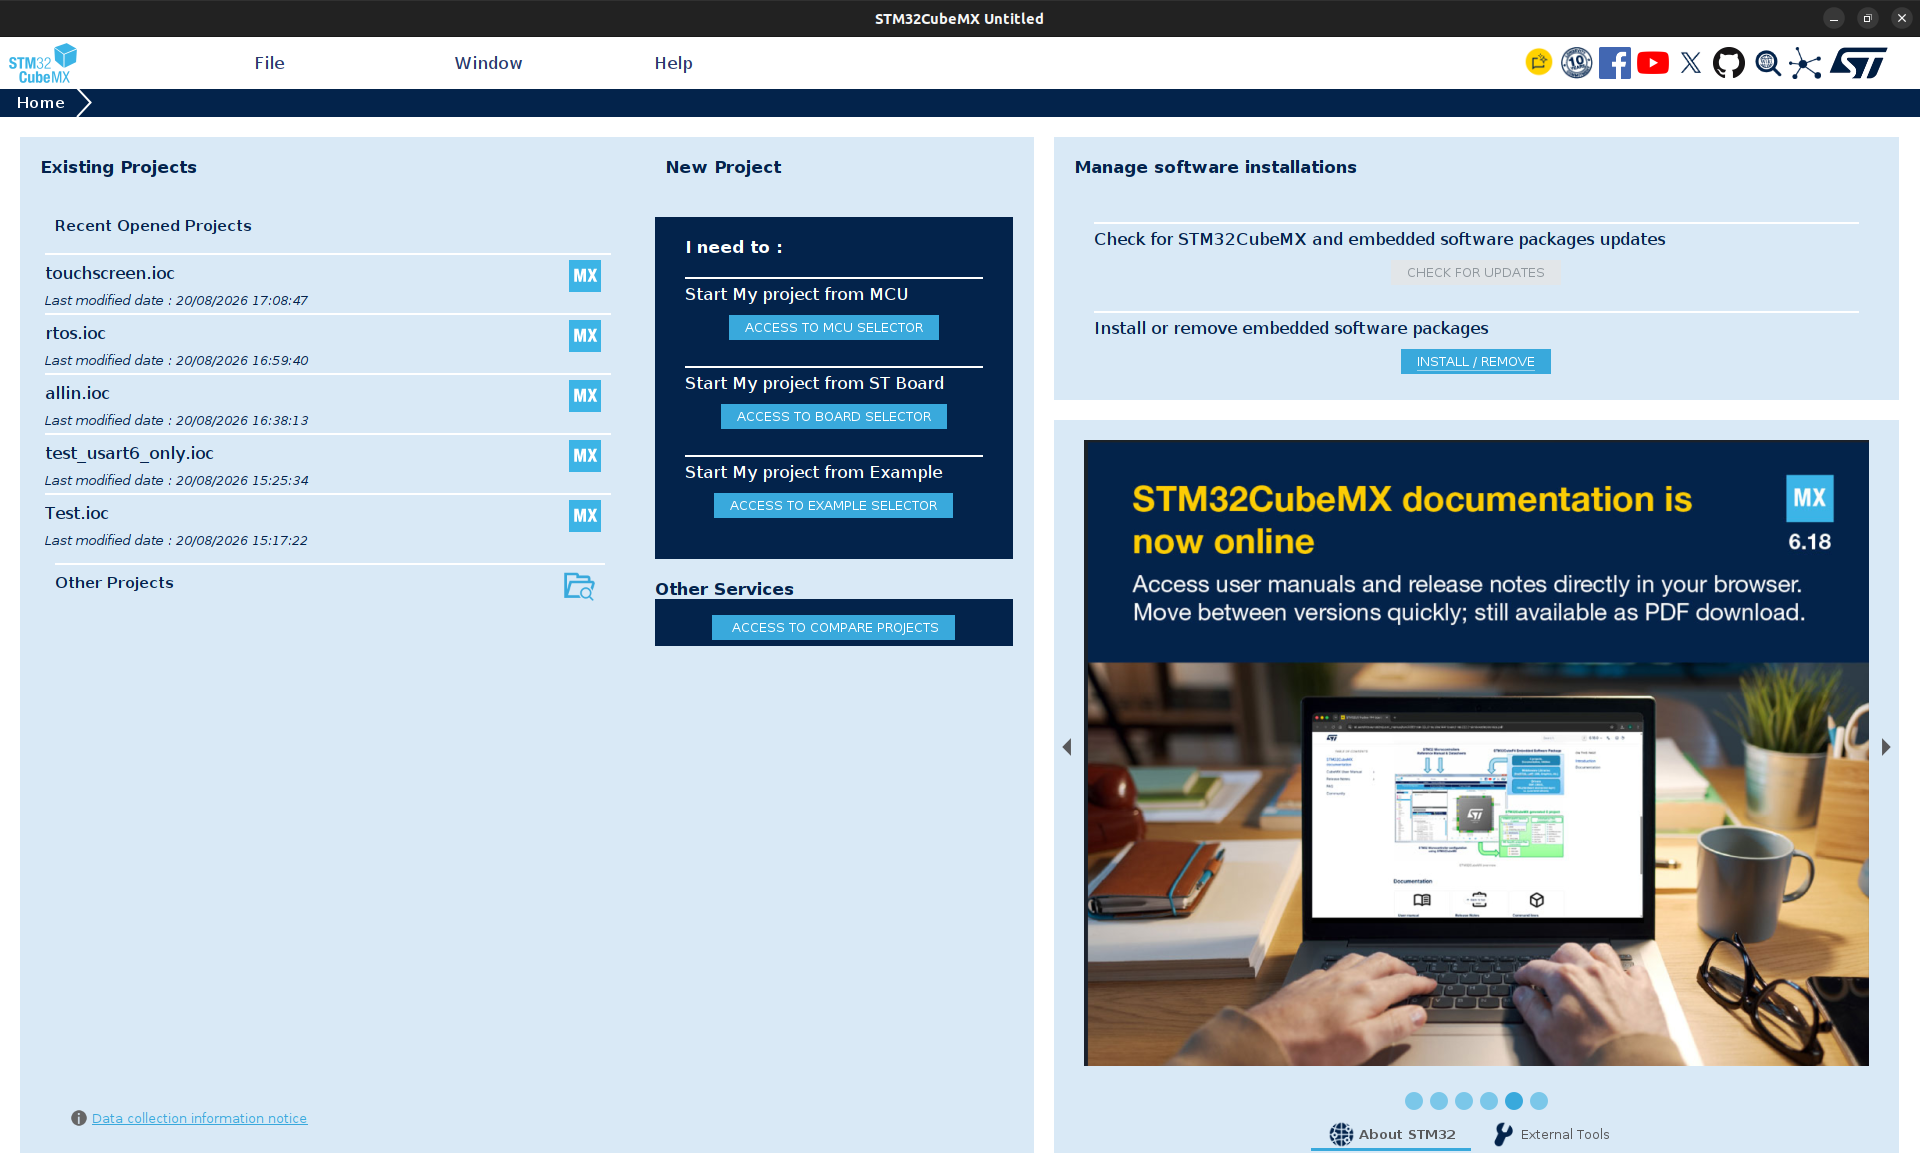
\includegraphics[width=\textwidth]{res/cubemx_00_init.png}
                \caption{Pantalla inicial de CubeMX}
                \label{fig:cubemx_00_init}
            \end{figure}

            Lo primero que haremos, si es que no está ya instalado, es descargar el paquete STM32F7 desde el apartado ``Install or remove embedded software packages'' (\Cref{fig:cubemx_01_package}).

            \begin{figure}
                \centering
                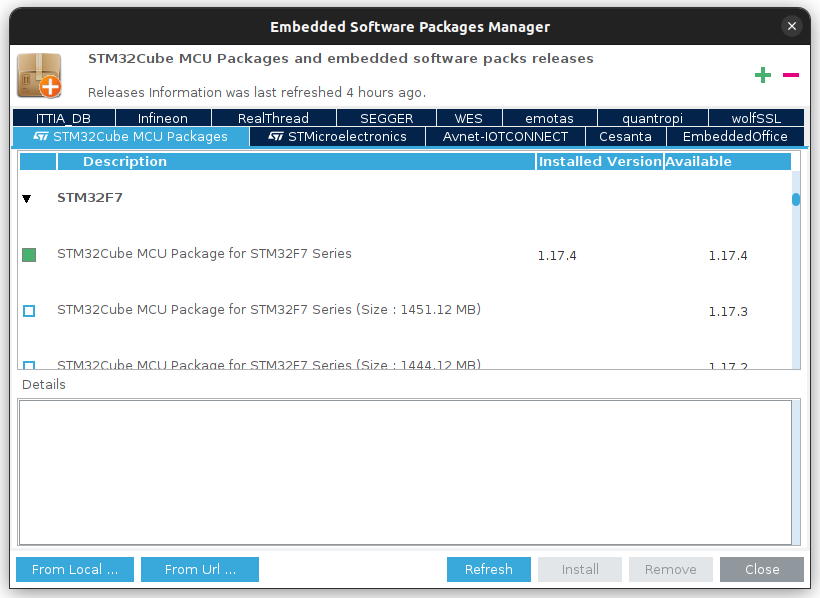
\includegraphics[width=0.8\textwidth]{res/cubemx_01_package.png}
                \caption{Instalación del paquete STM32F7}
                \label{fig:cubemx_01_package}
            \end{figure}

            A continuación, debemos elegir el componente base de nuestro proyecto. Tenemos dos opciones:
            \begin{itemize}
                \item \textbf{MCU}: Empieza el proyecto partiendo de un procesador sin ninguna conexión activa. En este modo, debemos asignar, a cada ``pata'' o pin del procesador una función concreta, planificando cómo lo soldaremos a una placa de prototipado a medida.
                \item \textbf{BOARD}: En este caso, partimos de un procesador que ya se encuentra dentro de una placa, y sus pines tienen conexiones concretas establecidas (LEDs, Botones, Pantallas...). En este modo, simplemente deberemos elegir qué funciones activamos, pero no tendremos la dificultad de tener que planificar qué hace cada pin. Utilizaremos este segundo modo eligiendo nuestra placa (723E discovery) (\Cref{fig:cubemx_02_boardselect}).
            \end{itemize} 

            \begin{figure}
                \centering
                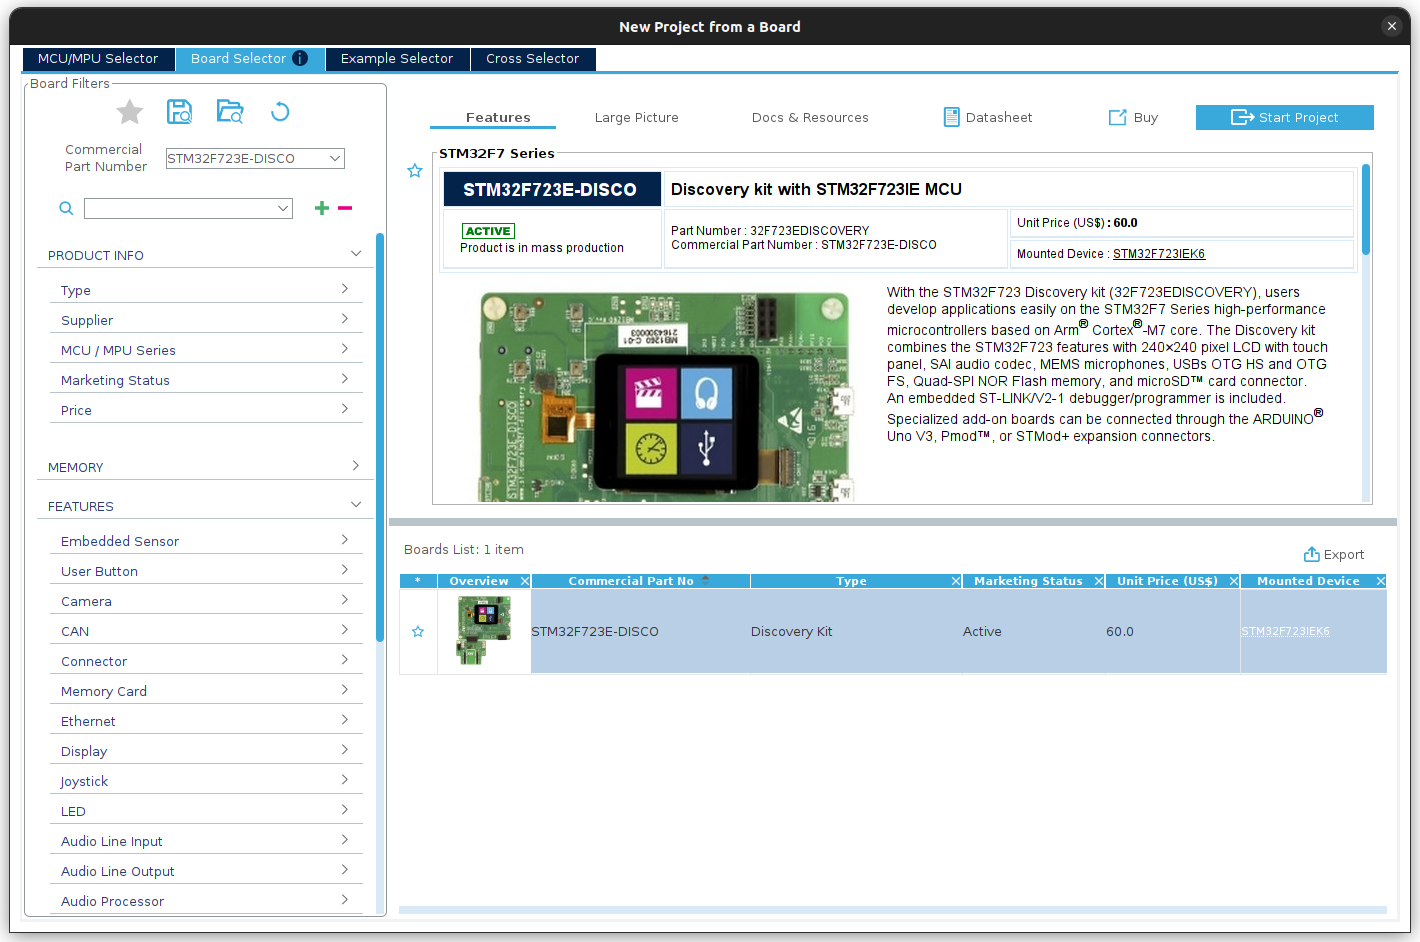
\includegraphics[width=\textwidth]{res/cubemx_02_boardselect.png}
                \caption{Selector de placas con la STM32F723E-DISCO seleccionada}
                \label{fig:cubemx_02_boardselect}
            \end{figure}

            Al crear el proyecto, nos pedirá una serie de opciones. En concreto, si queremos iniciar \textbf{TODOS} los periféricos (\Cref{fig:cubemx_03_peripheraldialog}, diremos que no), y si queremos preconfigurar la MPU (\Cref{fig:cubemx_04_memoryrecom}, diremos que sí). 

            Si quisiéramos habilitar TODA la funcionalidad de la placa, deberíamos decir que sí al primer diálogo, pero esto nos hará tener un paquete demasiado grande para las pruebas que queremos hacer.

            \begin{figure}
                \centering
                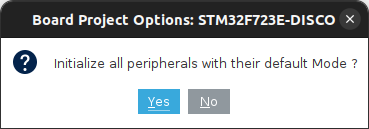
\includegraphics[width=0.4\textwidth]{res/cubemx_03_peripheraldialog.png}
                \caption{Diálogo de inicialización: seleccionar NO}
                \label{fig:cubemx_03_peripheraldialog}
            \end{figure}

            \begin{figure}
                \centering
                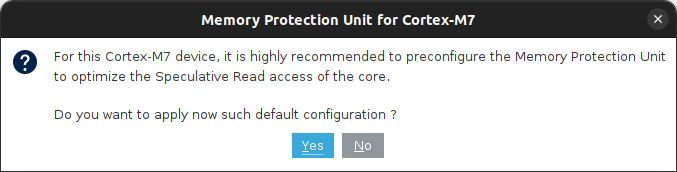
\includegraphics[width=0.7\textwidth]{res/cubemx_04_memoryrecom.png}
                \caption{Diálogo de configuración de memoria: seleccionar SÍ}
                \label{fig:cubemx_04_memoryrecom}
            \end{figure}

            Una vez creado el proyecto, podemos ver la planificación inicial en la \Cref{fig:cubemx_05_layout}: 
            \begin{itemize}
                \item Los pines color crema corresponden a alimentación (diferentes niveles de voltaje y tierra).
                \item Los pines color gris están deshabilitados (no conectados a ningún lado en la placa, por tanto no tienen uso).
                \item Los pines color verde caqui y aguamarina (solo solo unos pocos) corresponden a funciones de reseteo y la secuencia de arranque.
                \item Los pines amarillos corresponden a funciones desactivadas pero disponibles (se pueden ir activando como veremos a continuación).
                \item Los pines verdes corresponden a funciones ya activas y que utilizará nuestra aplicación.
            \end{itemize} 

            Hay que tener en cuenta que esta configuración de pines es la que se generará automáticamente por la herramienta, lo cual no quita que nosotros podamos cambiarla ``al vuelo'' dentro de nuestra aplicación, mediante acceso a todos los registros correspondientes de \PER{GPIO}.

            \begin{figure}
                \centering
                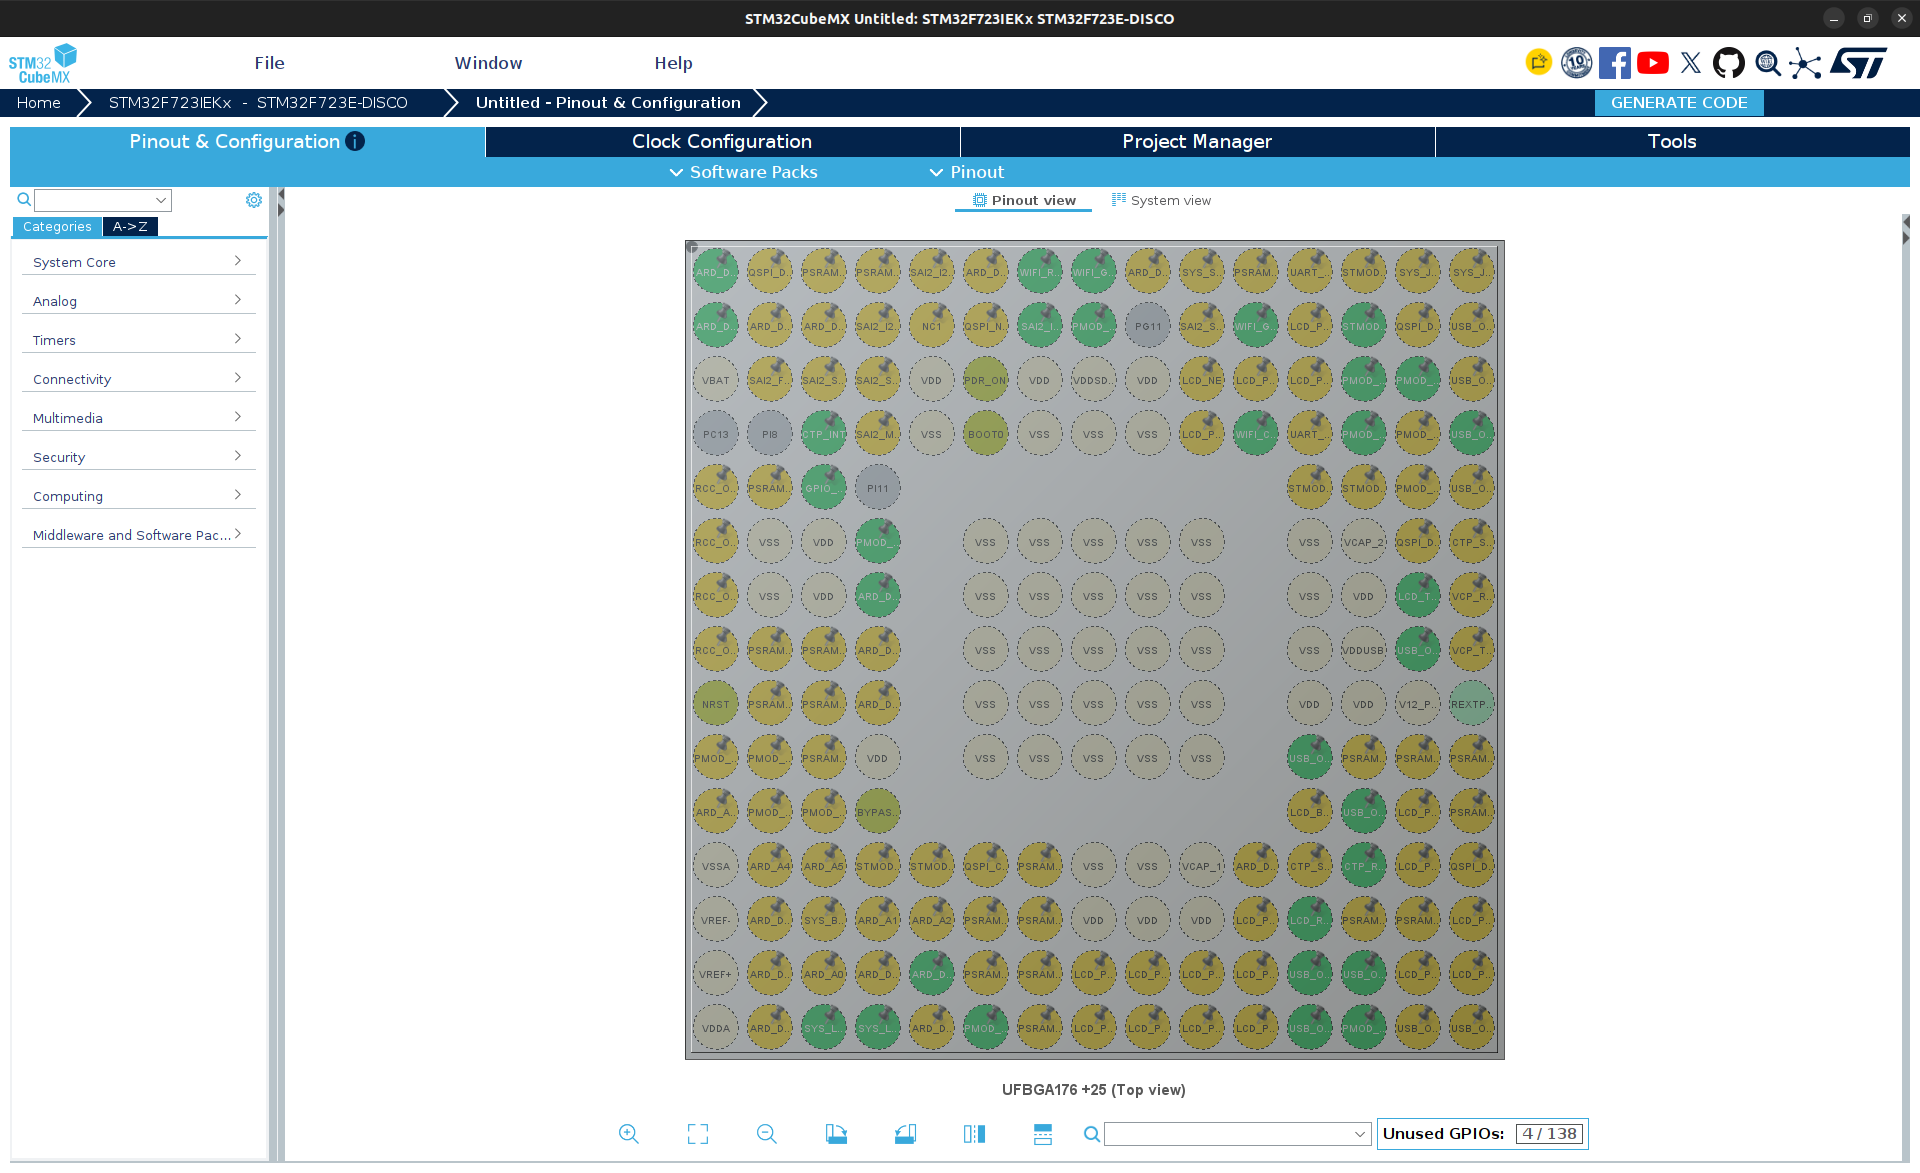
\includegraphics[width=\textwidth]{res/cubemx_05_layout.png}
                \caption{Disposición inicial del procesador en cubemx. Se observan todos los pines y sus funciones}
                \label{fig:cubemx_05_layout}
            \end{figure}

            Para esta práctica vamos a hacer un par de cambios. El primero es cambiar la función del pin \texttt{PA0} para que dispare una interrupción. Deberemos pinchar en él (es el de la posición (3,3) empezando por la esquina inferior izquierda), y seleccionar \texttt{GPIO\_EXTI0} para habilitar su función de interrupción externa (\Cref{fig:cubemx_06_pinchange}). Finalmente tendremos también que seleccionar la generación de interrupción desde \PER{NVIC} en el menú correspondiente (\Cref{fig:cubemx_07_nviceint0}).

            \begin{figure}
                \centering
                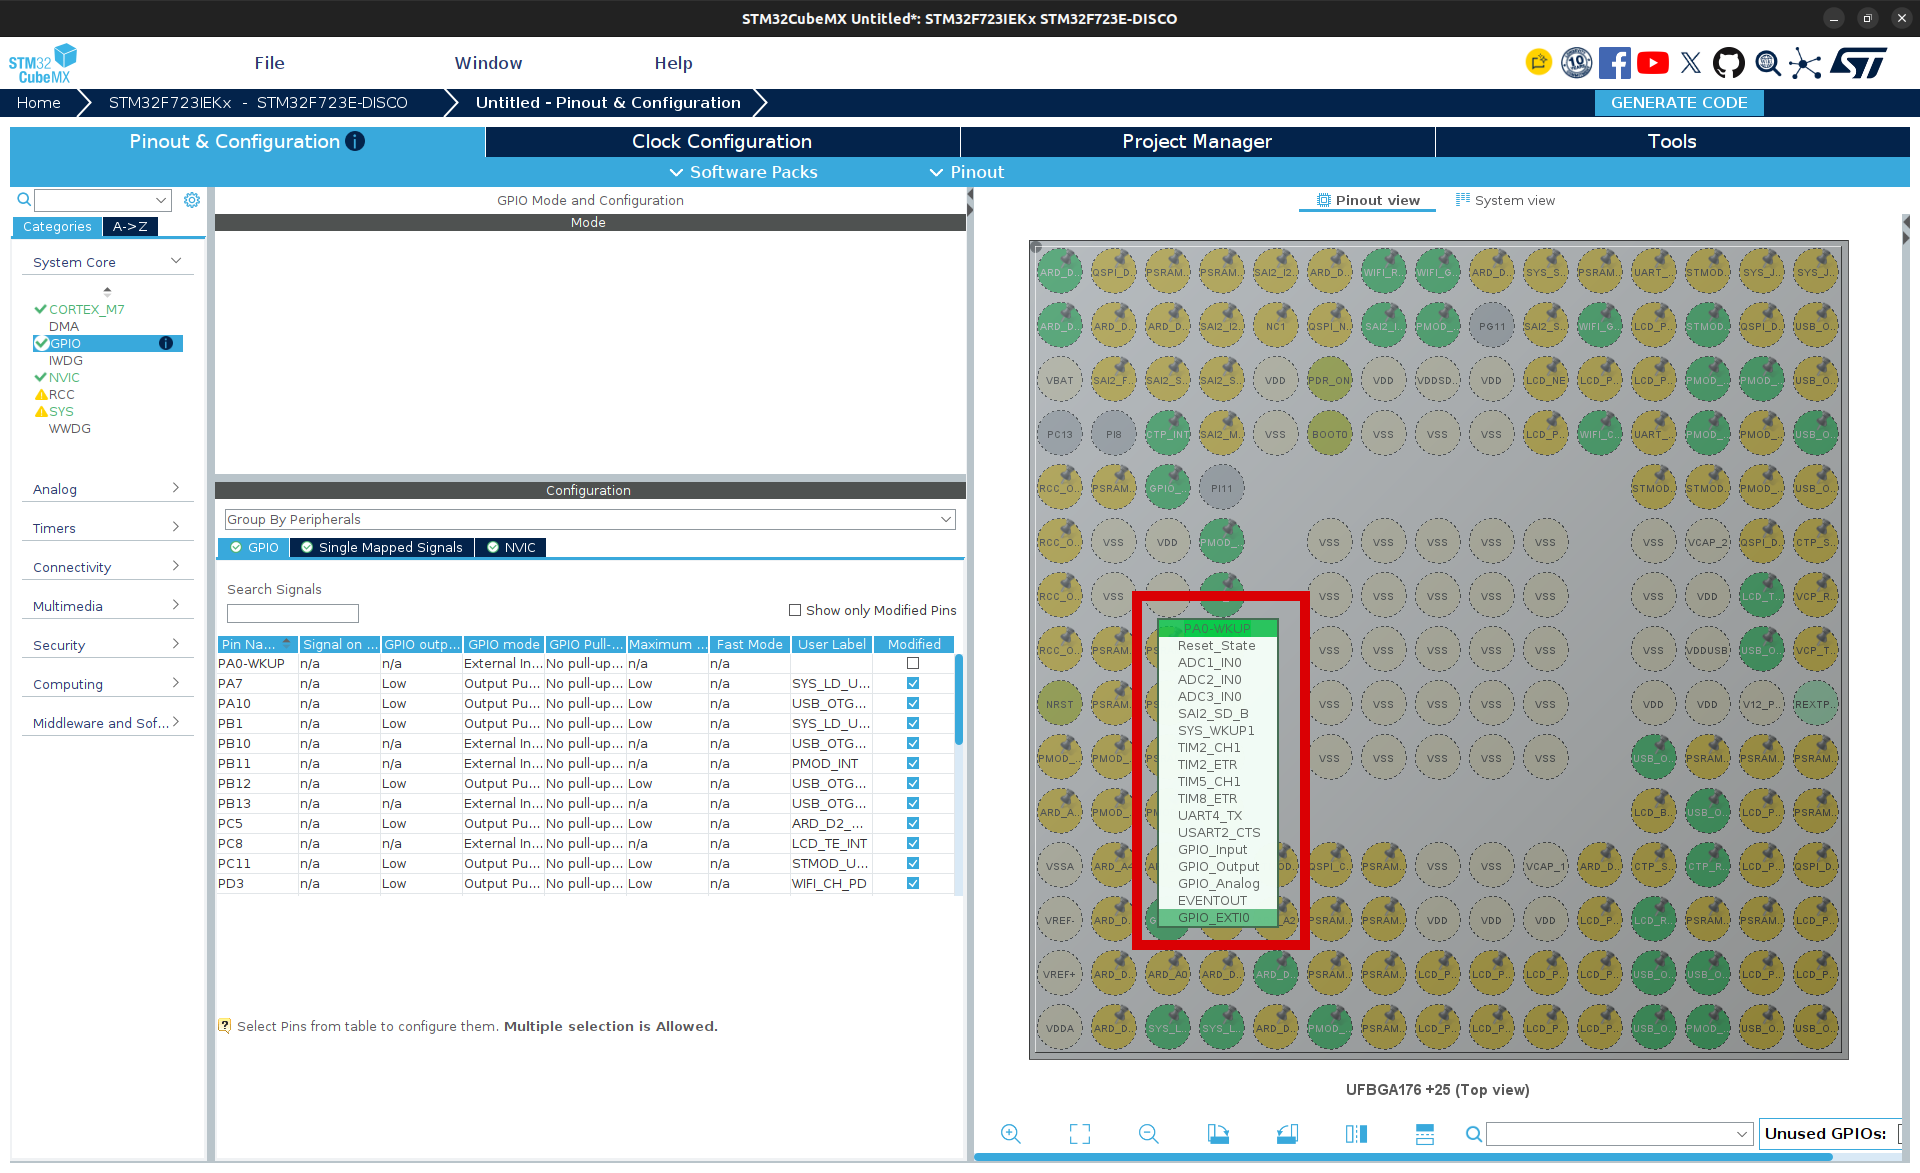
\includegraphics[width=\textwidth]{res/cubemx_06_pinchange.png}
                \caption{Cambio de función de un pin}
                \label{fig:cubemx_06_pinchange}
            \end{figure}

            \begin{figure}
                \centering
                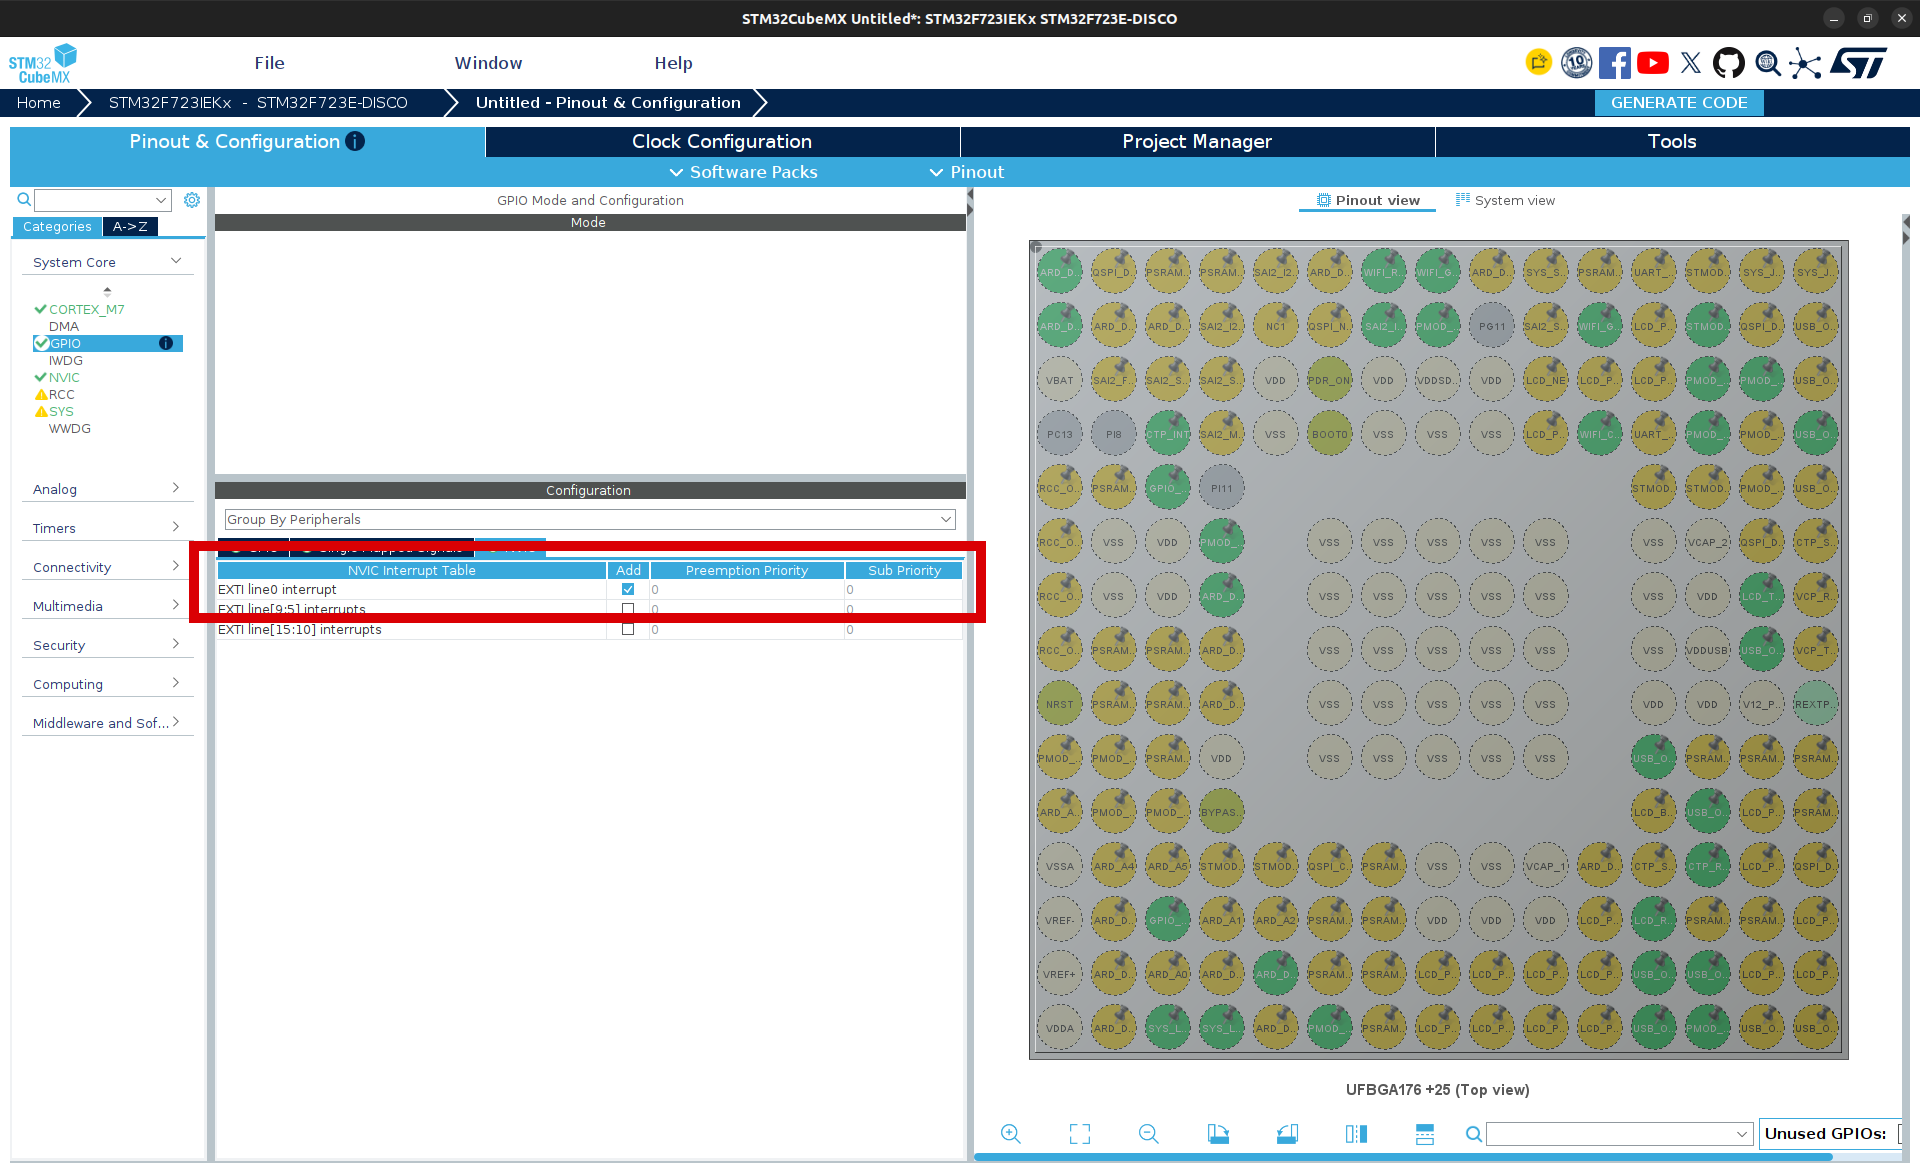
\includegraphics[width=\textwidth]{res/cubemx_07_nviceint0.png}
                \caption{Activación de interrupciones para el pin de \PER{GPIO} A0}
                \label{fig:cubemx_07_nviceint0}
            \end{figure}

            Además de tratar con los pines, podemos realizar la configuración de todos los periféricos que contiene el procesador. En la barra lateral izquierda, los veremos categorizados. Vamos a activar la \PER{UART6} para poder enviar mensajes al ordenador a través de la conexión serie. Para ello, tenemos que seleccionar en la lista \texttt{Connectivity > USART6} y luego activarla poniéndola en modo \texttt{Asyncrhonous} (\Cref{fig:cubemx_08_usart6}).

            Veremos que numerosos periféricos y opciones aparecen en color rojo/rosa. Esto es porque la herramienta detecta configuraciones incompatibles que no nos deja cambiar. (Imaginemos por ejemplo que la UART y el bus I2C comparten pines, sólo podríamos tener habilitado uno). Si queremos ver por qué una opción está deshabilitada, basta con dejar el ratón encima, y nos dirá que otras funcionalidades entran en conflicto.

            \begin{figure}
                \centering
                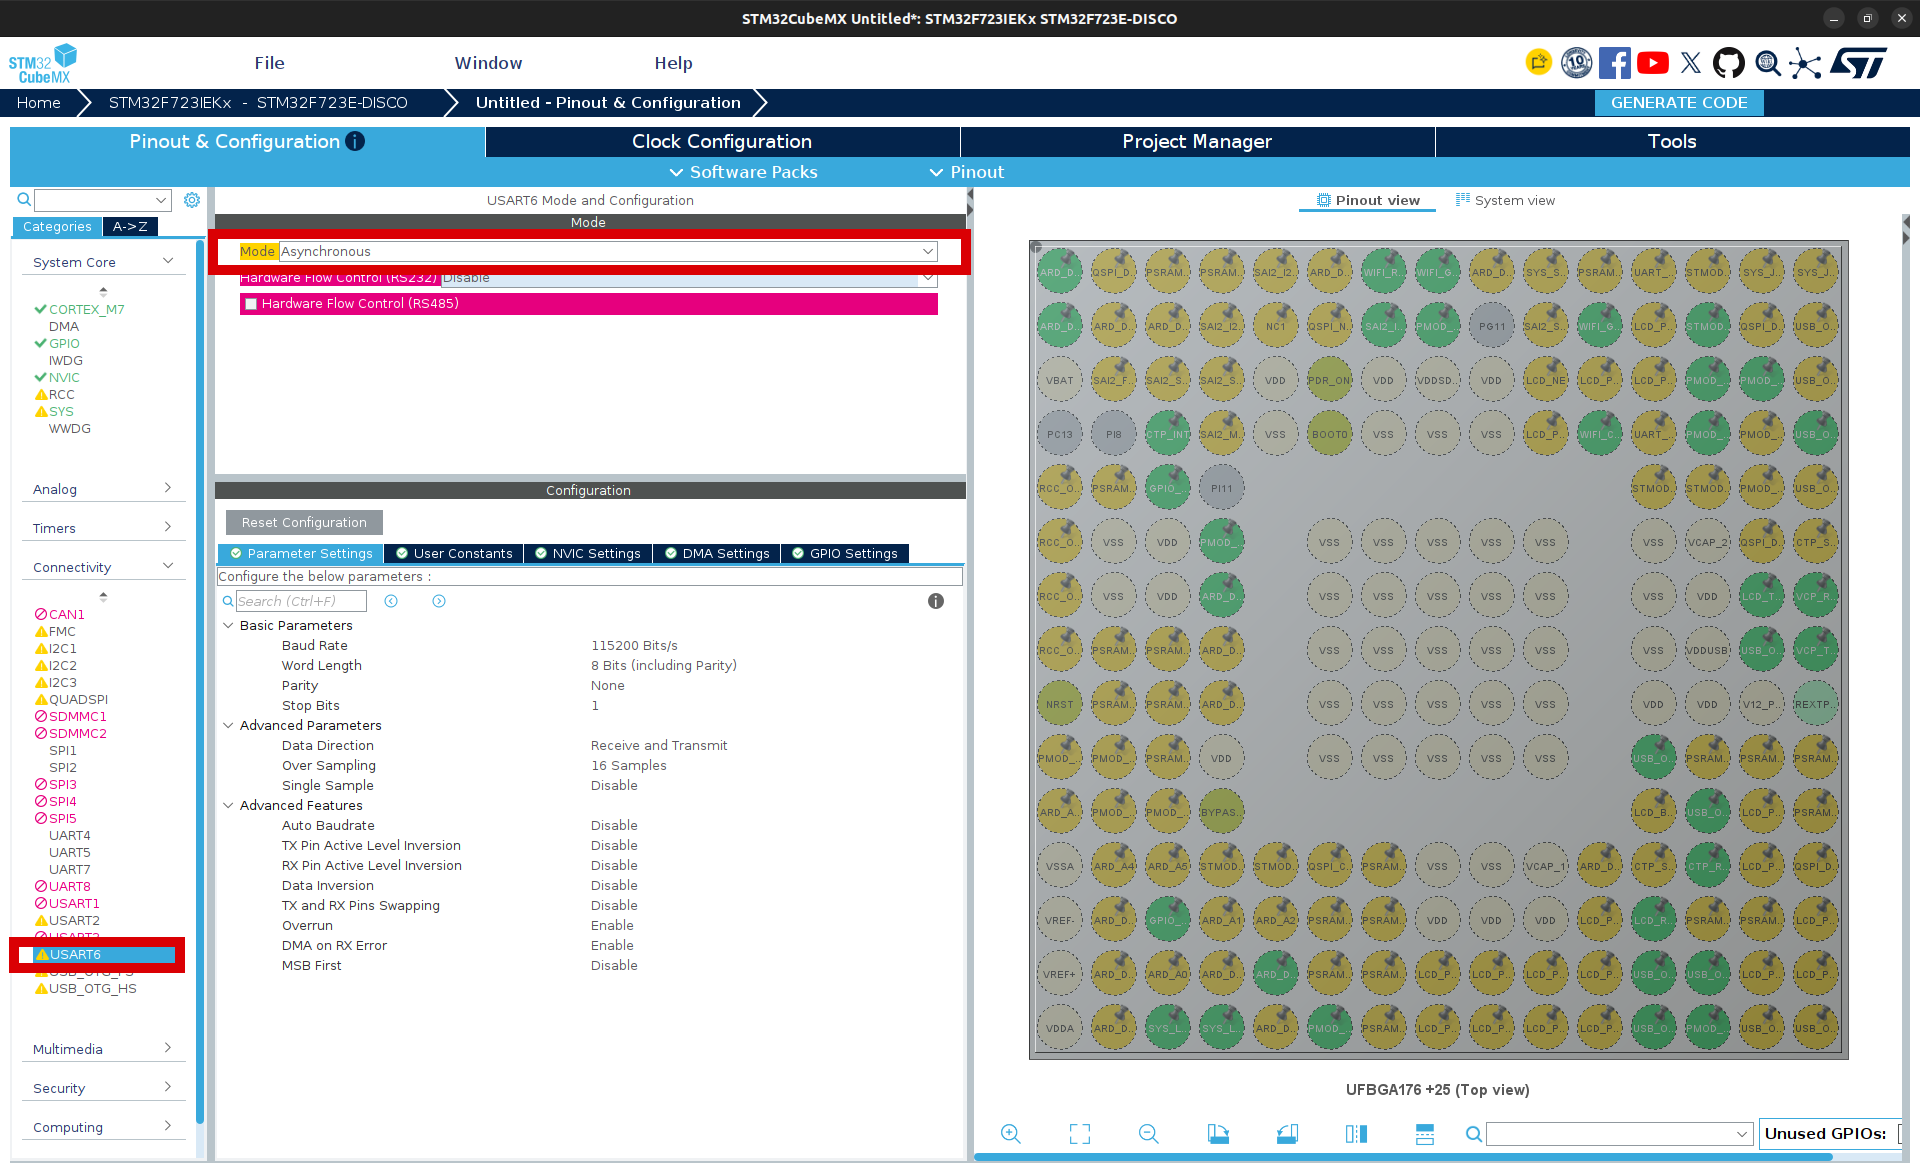
\includegraphics[width=\textwidth]{res/cubemx_08_usart6.png}
                \caption{Activación del periférico \PER{USART6}}
                \label{fig:cubemx_08_usart6}
            \end{figure}

            Otra parte bastante potente y que podemos configurar aquí es la gestión del árbol de relojes (\Cref{fig:cubemx_09_clock}). El árbol de relojes es la estructura del procesador que toma la oscilación inicial de un cristal o bucle de inversores, y genera frecuencias concretas para todos los elementos internos del procesador. En otras prácticas no hemos estado modificando su configuración, y el reloj por defecto era de 16MHz. Aquí podemos ver que, utilizando diversos multiplicadores y divisores de frecuencia, se consigue un reloj objetivo de 216MHz. Su configuración se generará automáticamente para la placa. Podemos probar a cambiar funciones para ver cómo afecta a todos los relojes del árbol. 
            
            Hay que tener en cuenta que, para la configuración de periféricos con reloj propio (como la UART), debemos saber con exactitud la frecuencia de referencia que reciben (por ejemplo, para ajustar valores de contadores), así que un cambio en este punto puede suponer un cambio en nuestro código.

            \begin{figure}
                \centering
                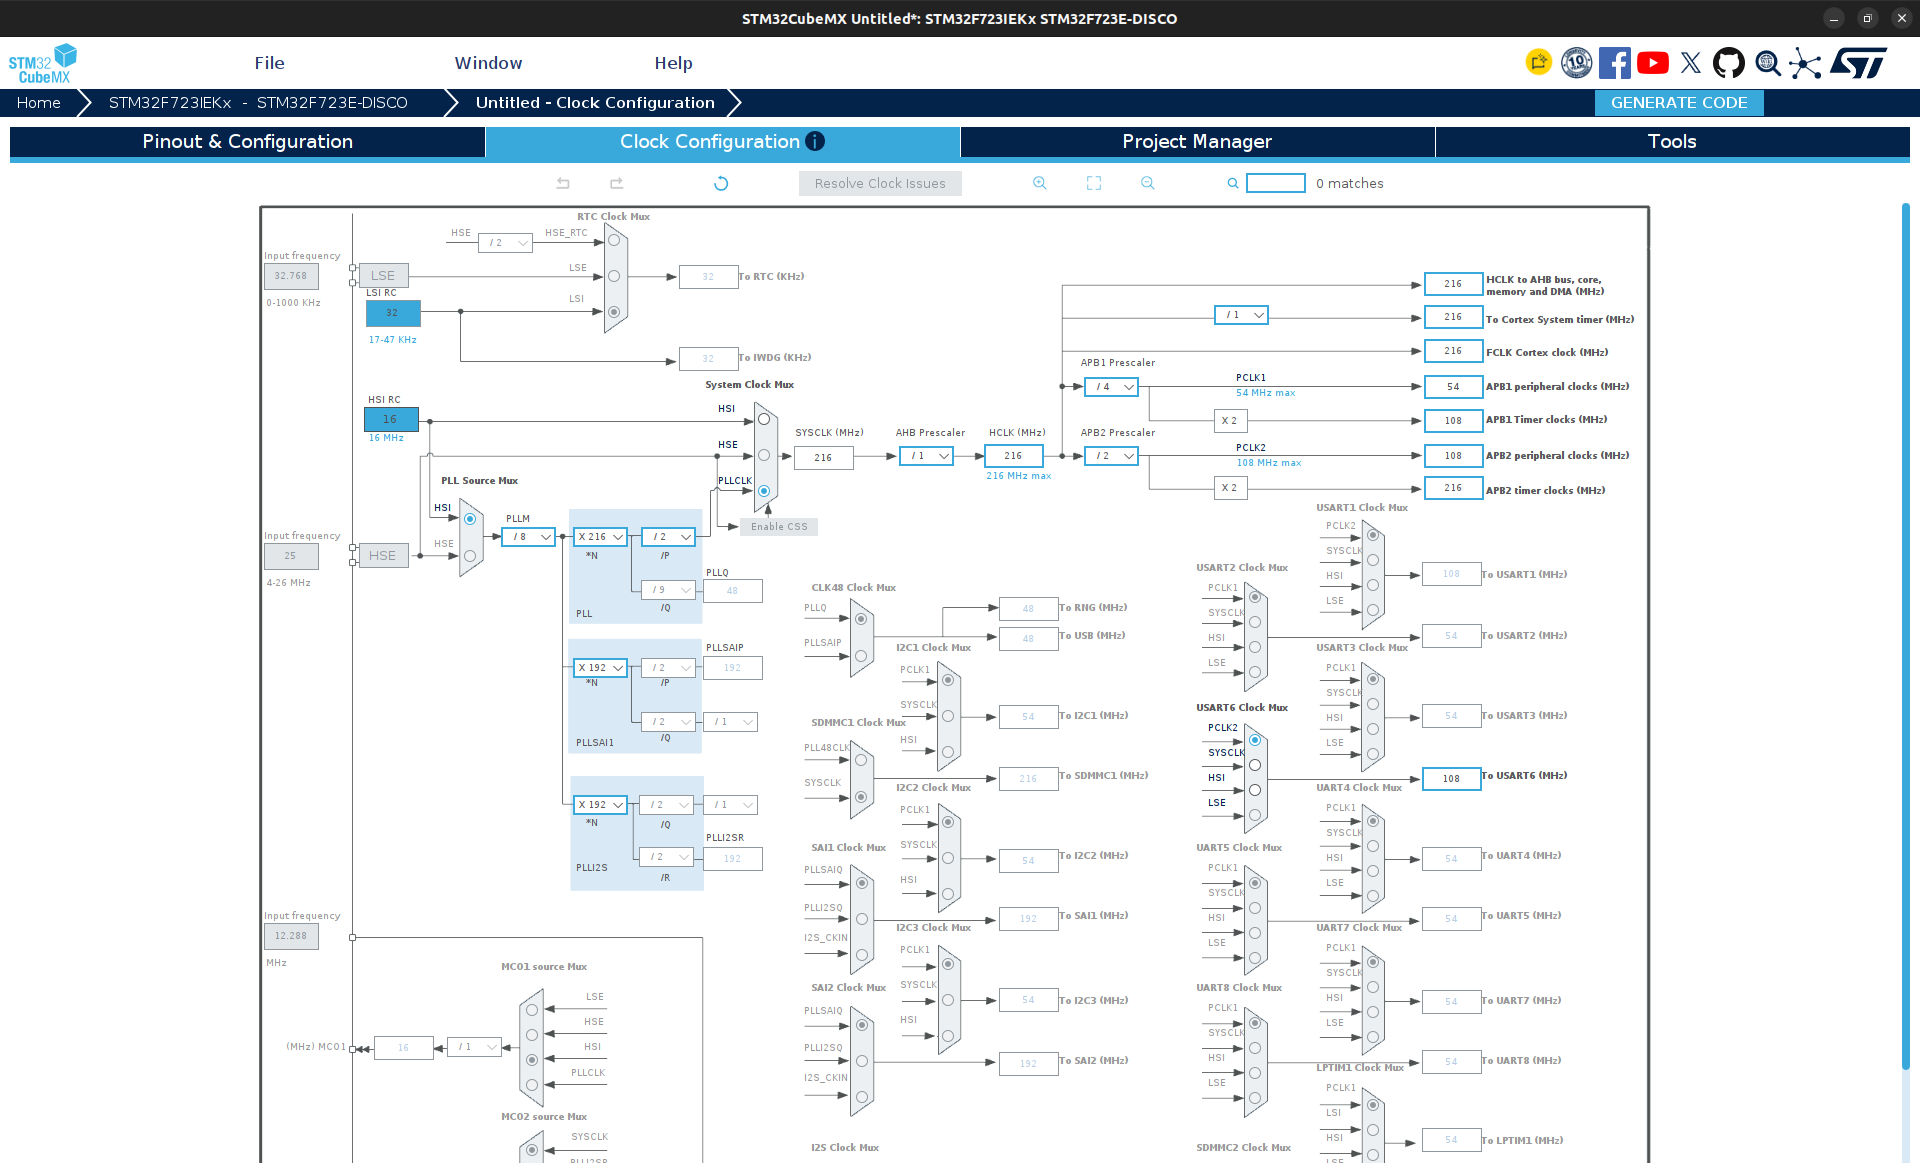
\includegraphics[width=\textwidth]{res/cubemx_09_clock.png}
                \caption{Configuración del reloj}
                \label{fig:cubemx_09_clock}
            \end{figure}

            Finalmente, estamos listos para generar el proyecto con nuestro BSP customizado, que incluirá la configuración ya hecha de los periféricos seleccionados y del árbol de reloj. Debemos dar un nombre y carpeta al proyecto, además de indicar que lo abriremos con STMCubeIDE (\Cref{fig:cubemx_10_project}). Una vez generado, nos dará la opción directamente de abrir el proyecto (\Cref{fig:cubemx_11_output}).

            \begin{figure}
                \centering
                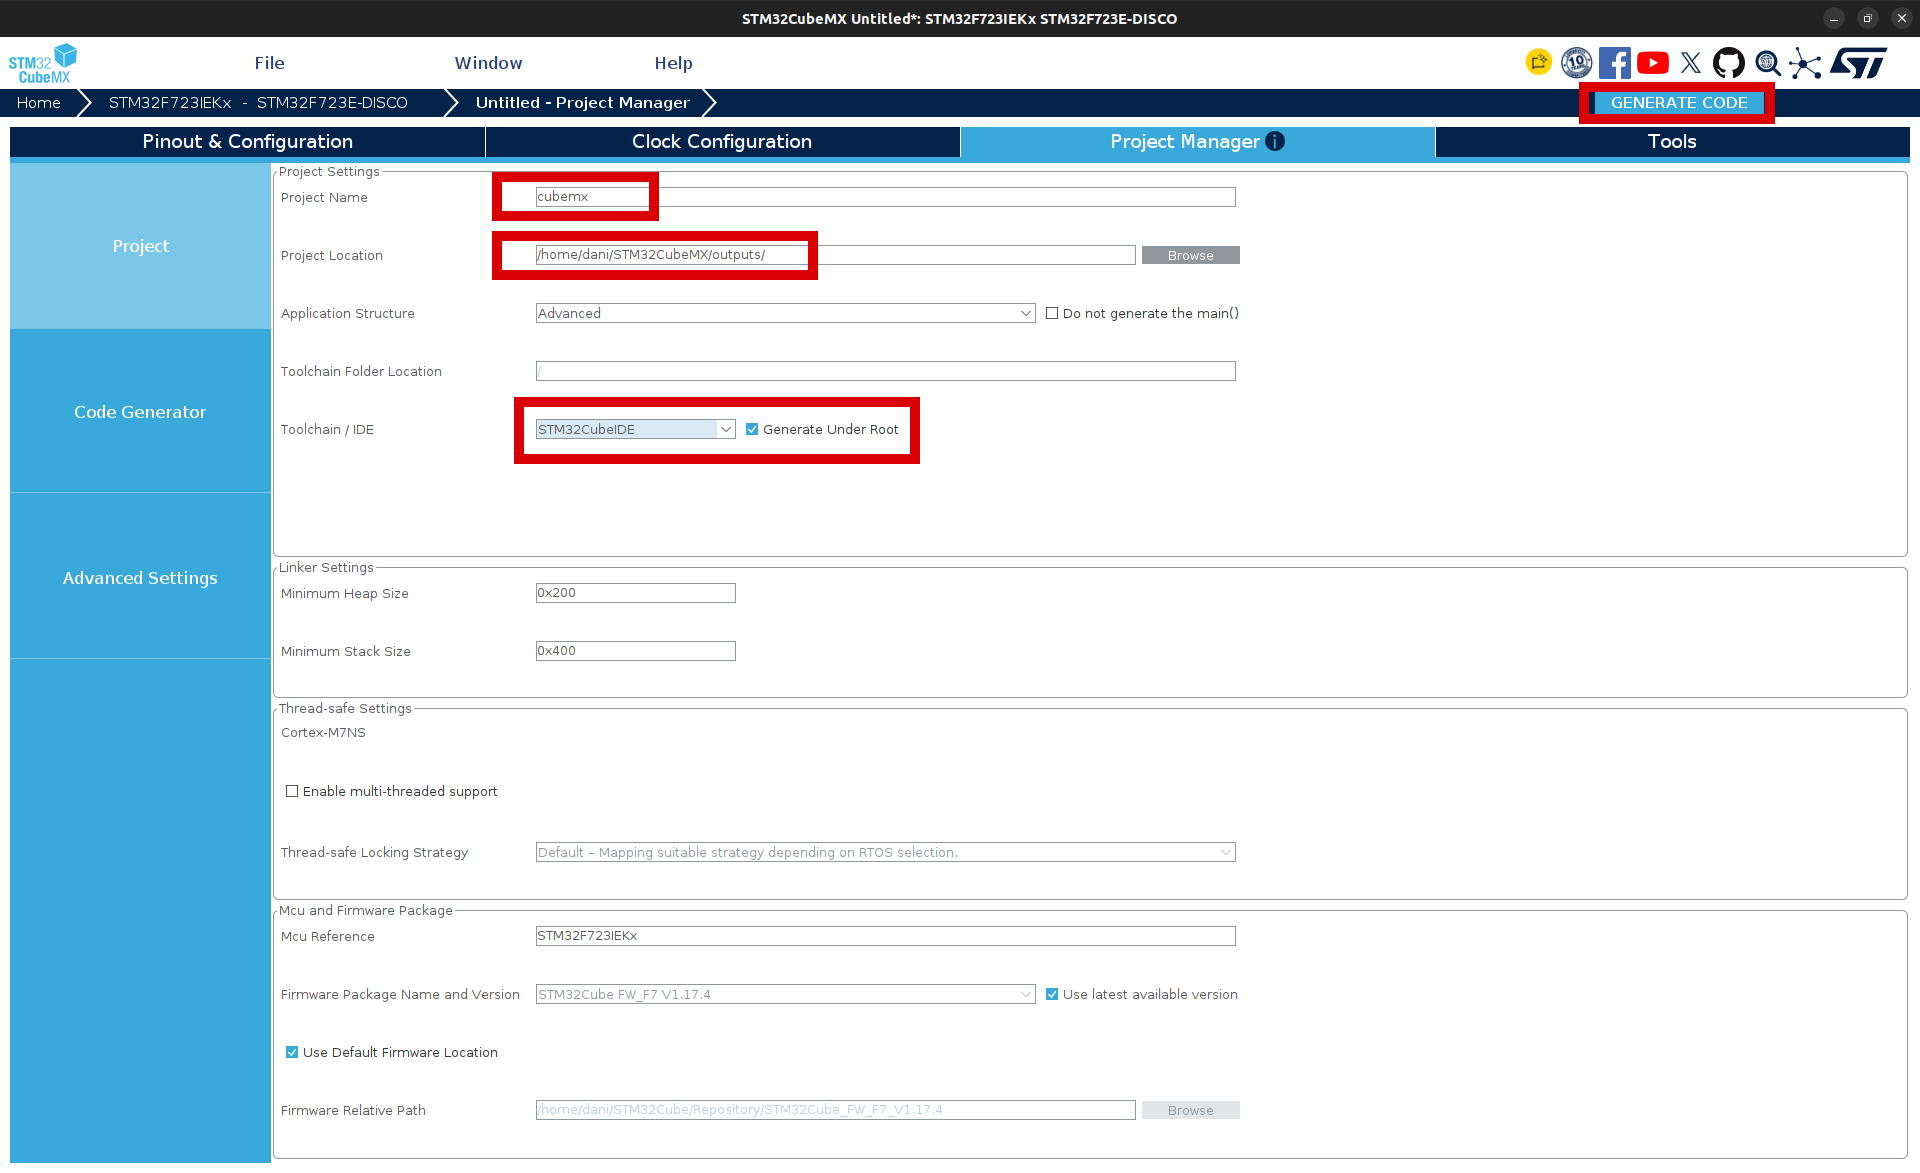
\includegraphics[width=\textwidth]{res/cubemx_10_project.png}
                \caption{Creación del proyecto con BSP para STMCubeIDE}
                \label{fig:cubemx_10_project}
            \end{figure}

            \begin{figure}
                \centering
                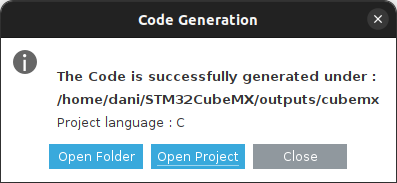
\includegraphics[width=0.5\textwidth]{res/cubemx_11_output.png}
                \caption{Diálogo de finalización. Seleccionar ``Open Project''}
                \label{fig:cubemx_11_output}
            \end{figure}

        \subsubsection{Uso del BSP desde STMCubeIDE}

            Ahora ya volvemos al familiar STMCubeIDE. Deberíamos haber visto un diálogo de importación correcta como el de la \Cref{fig:cubeide_01_import}.

            \begin{figure}
                \centering
                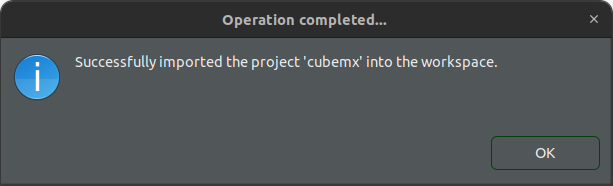
\includegraphics[width=0.7\textwidth]{res/cubeide_01_import.png}
                \caption{Diálogo de importación exitosa en STMCubeIDE}
                \label{fig:cubeide_01_import}
            \end{figure}

            En la \Cref{fig:cubeide_02_main} vemos la estructura de ficheros, así como el código automáticamente generado para la función \texttt{main}, que inicializa la MPU, reloj, y periféricos activados (En nuestro caso, algunas inicializaciones genéricas, además de los \PER{GPIO} y \PER{USART6}).

            \begin{figure}
                \centering
                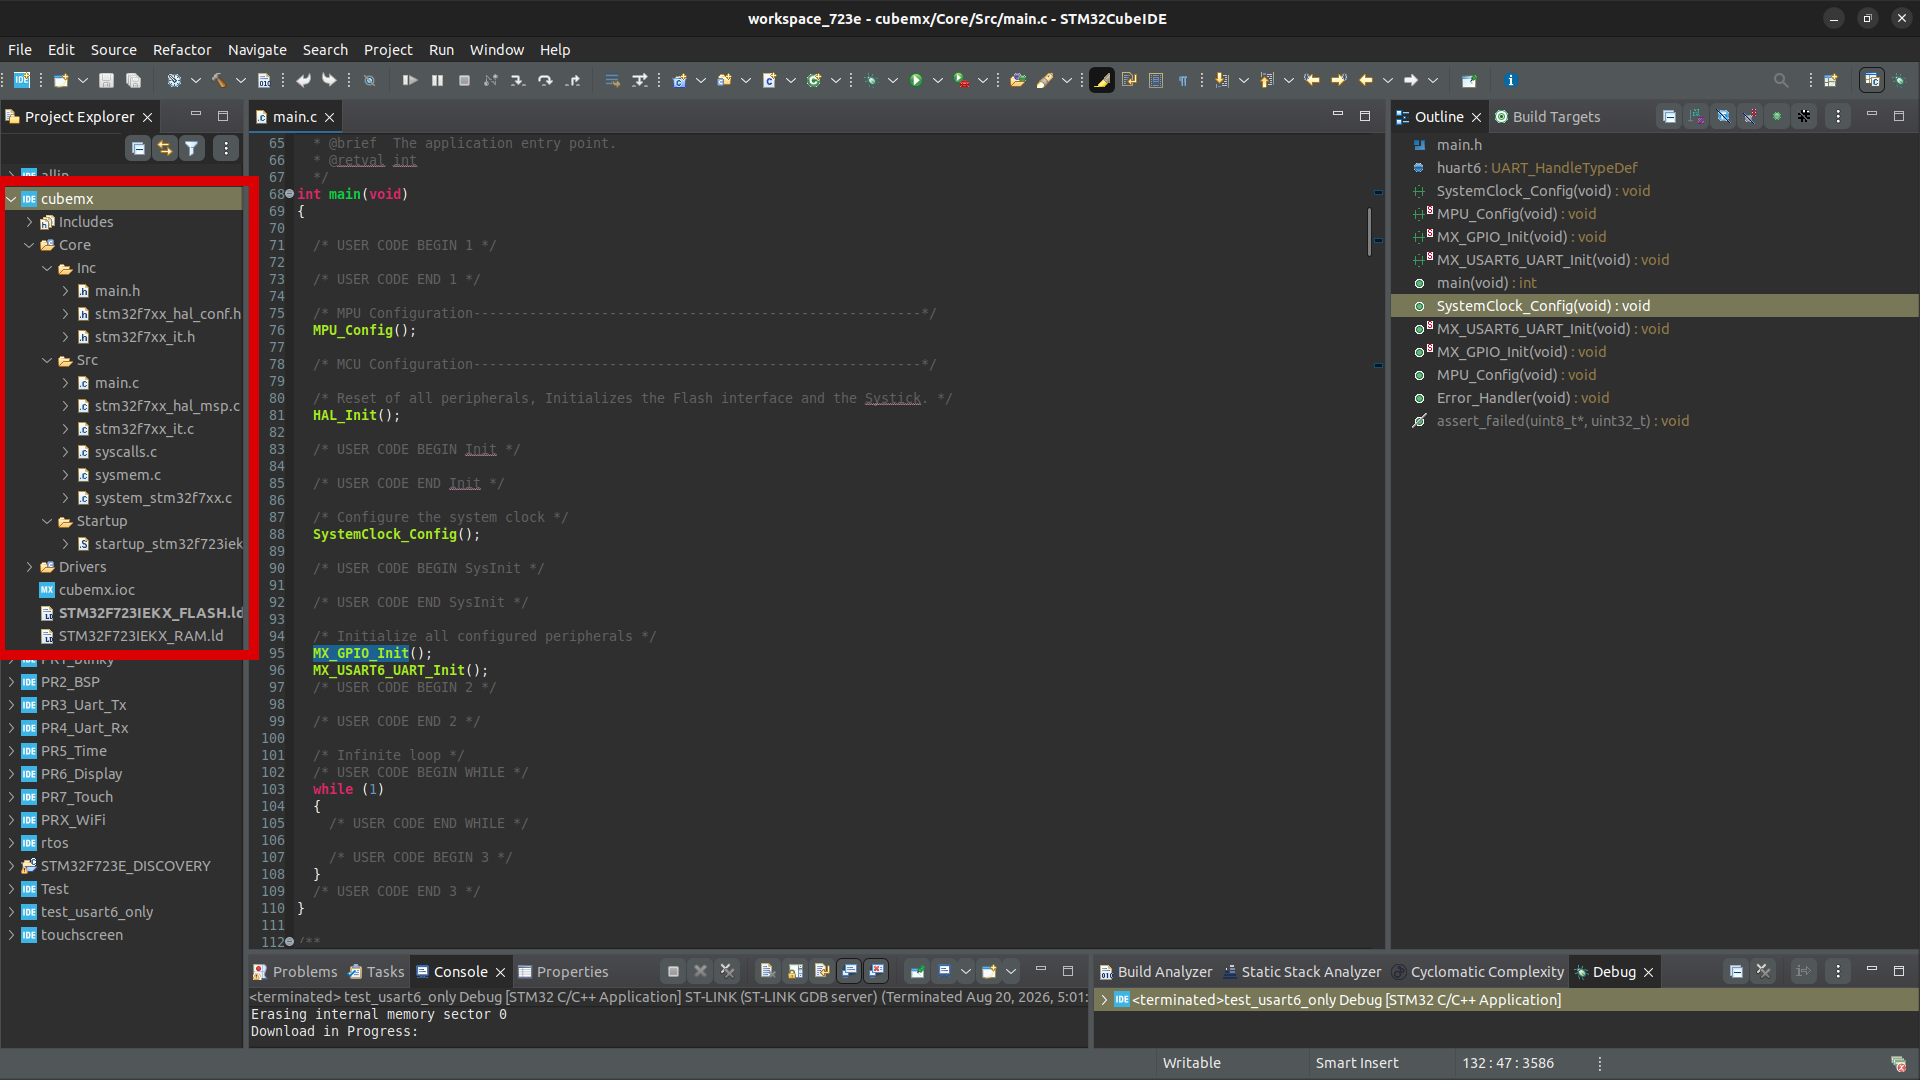
\includegraphics[width=\textwidth]{res/cubeide_02_main.png}
                \caption{Estructura del proyecto creado y código main}
                \label{fig:cubeide_02_main}
            \end{figure}

            En la \Cref{fig:cubeide_03_clock} podemos ver el código de inicialización del reloj. Una cosa interesante a observar en este BSP, es que suele tener estructuras de configuración complejas (\texttt{RCC\_OscInitStruct}) que luego ya se vuelcan en registros internos (en este caso del \PER{RCC}) de golpe en las funciones internas.

            \begin{figure}
                \centering
                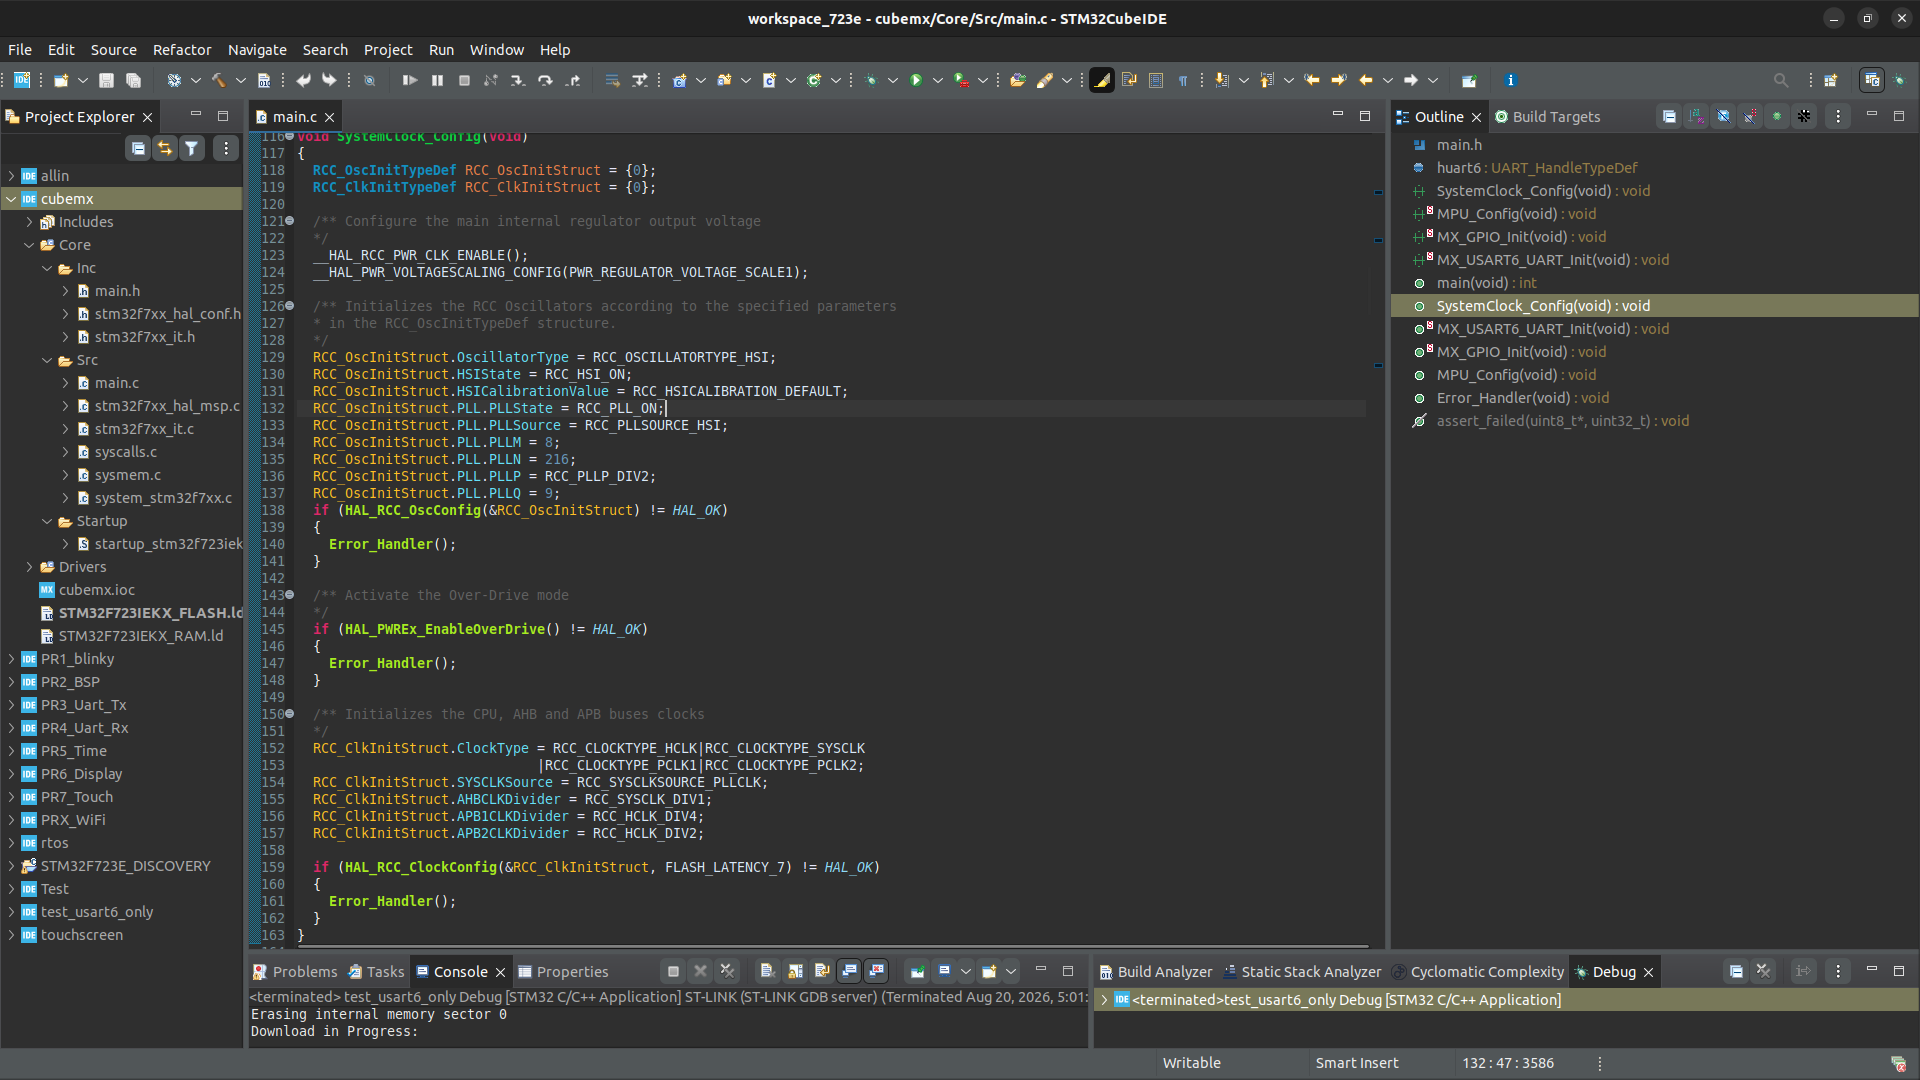
\includegraphics[width=\textwidth]{res/cubeide_03_clock.png}
                \caption{Código creado para inicializar el reloj}
                \label{fig:cubeide_03_clock}
            \end{figure}

            Para las interrupciones, por ejemplo, vemos que configura el \PER{NVIC} en la \Cref{fig:cubeide_04_interrupt}, y genera el manejador de interrupción en \Cref{fig:cubeide_05_interrupt}. En este caso, por darnos mayor abstracción, ya gestiona automáticamente el borrado de la interrupción pendiente, y nos ofrece una función \texttt{\_\_weak} que podemos sobreescribir en nuestro fichero \texttt{main.c} para capturar la interrupción.

            \begin{figure}
                \centering
                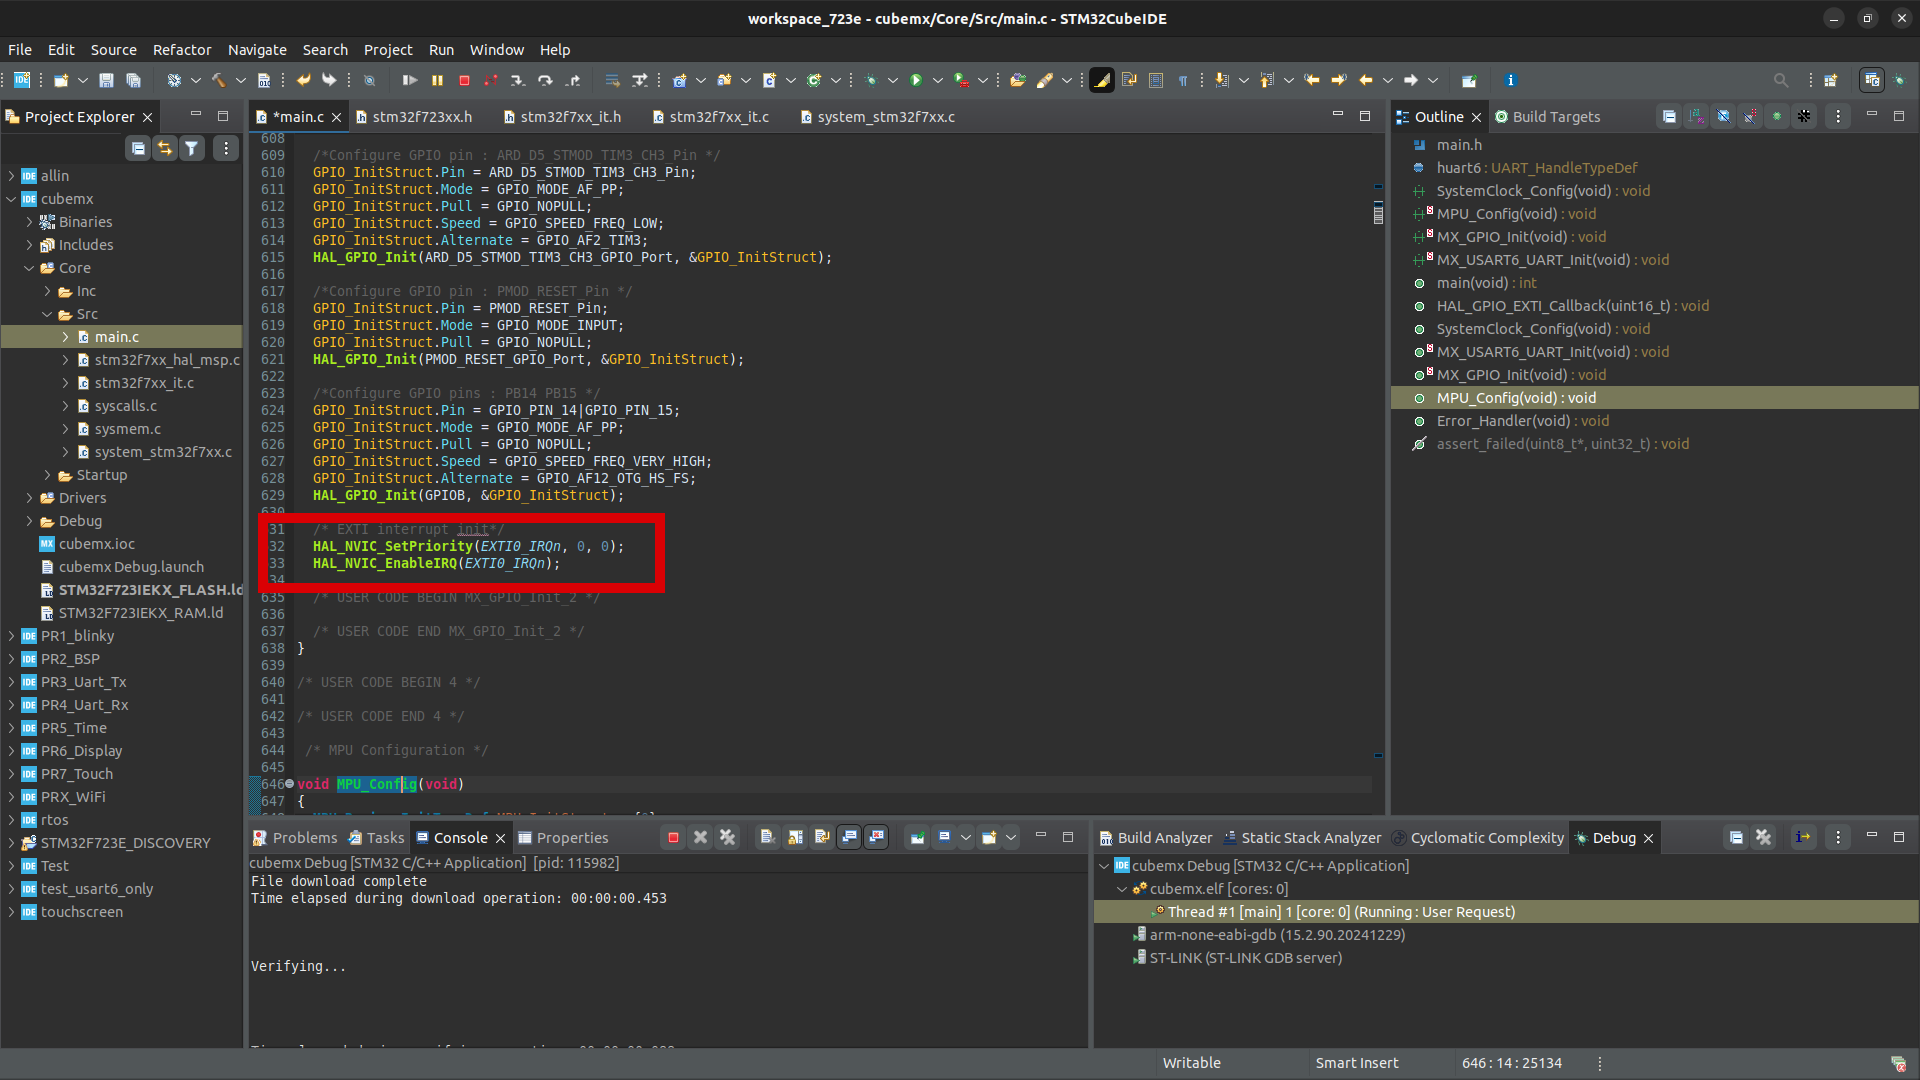
\includegraphics[width=\textwidth]{res/cubeide_04_interrupt.png}
                \caption{Código generado para inicializar las interrupciones}
                \label{fig:cubeide_04_interrupt}
            \end{figure}

            \begin{figure}
                \centering
                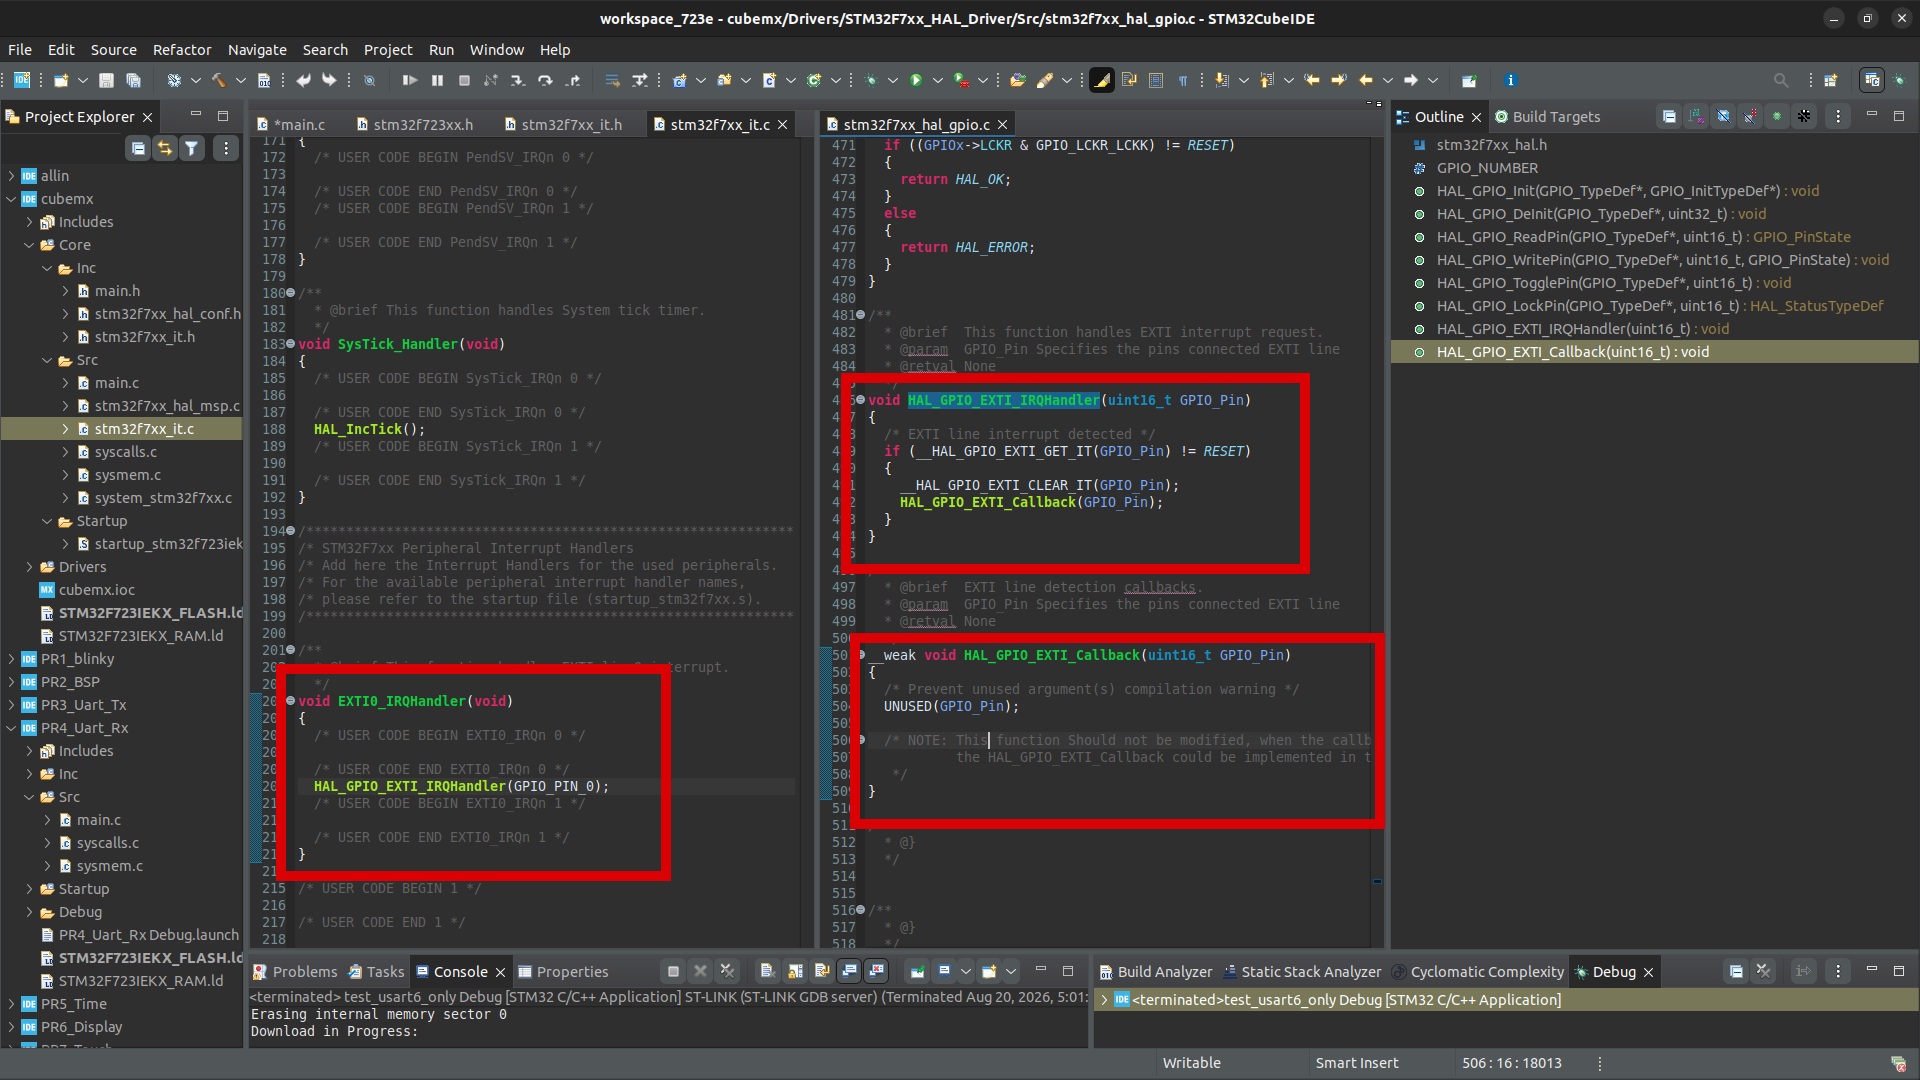
\includegraphics[width=\textwidth]{res/cubeide_05_interrupt.png}
                \caption{Estructura de las interrupciones, se ofrece mediante un \emph{callback} al usuario}
                \label{fig:cubeide_05_interrupt}
            \end{figure}

            También vemos cómo ha realizado la configuración de los pines del LED (ya configurado por defecto) (\Cref{fig:cubeide_06_ledpinsetup}) y del botón (\Cref{fig:cubeide_07_btnpinsetup}). También configura multitud de pines extra (para todos los periféricos) aunque no les esté dando uso, ya que no los desactivamos en la vista de \emph{pinout}.

            \begin{figure}
                \centering
                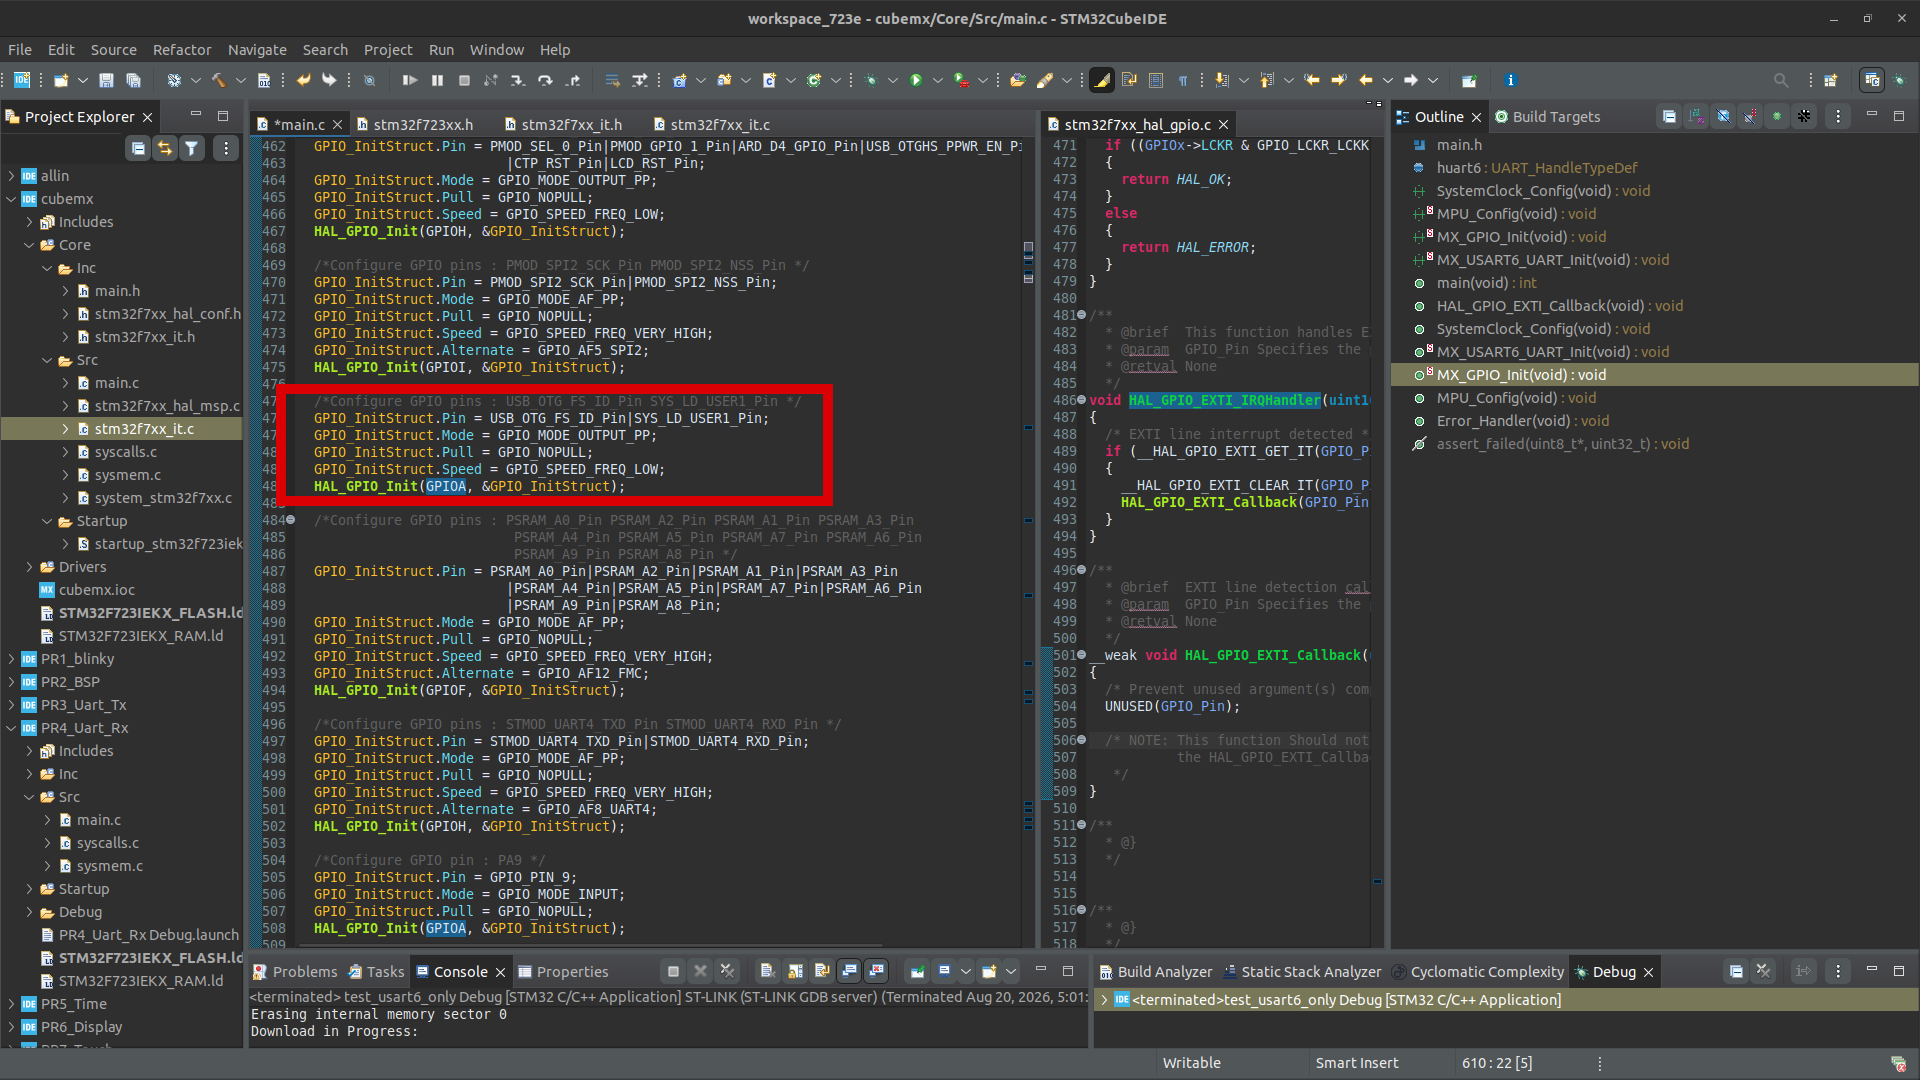
\includegraphics[width=\textwidth]{res/cubeide_06_ledpinsetup.png}
                \caption{Configuración automática del pin para el LED}
                \label{fig:cubeide_06_ledpinsetup}
            \end{figure}

            \begin{figure}
                \centering
                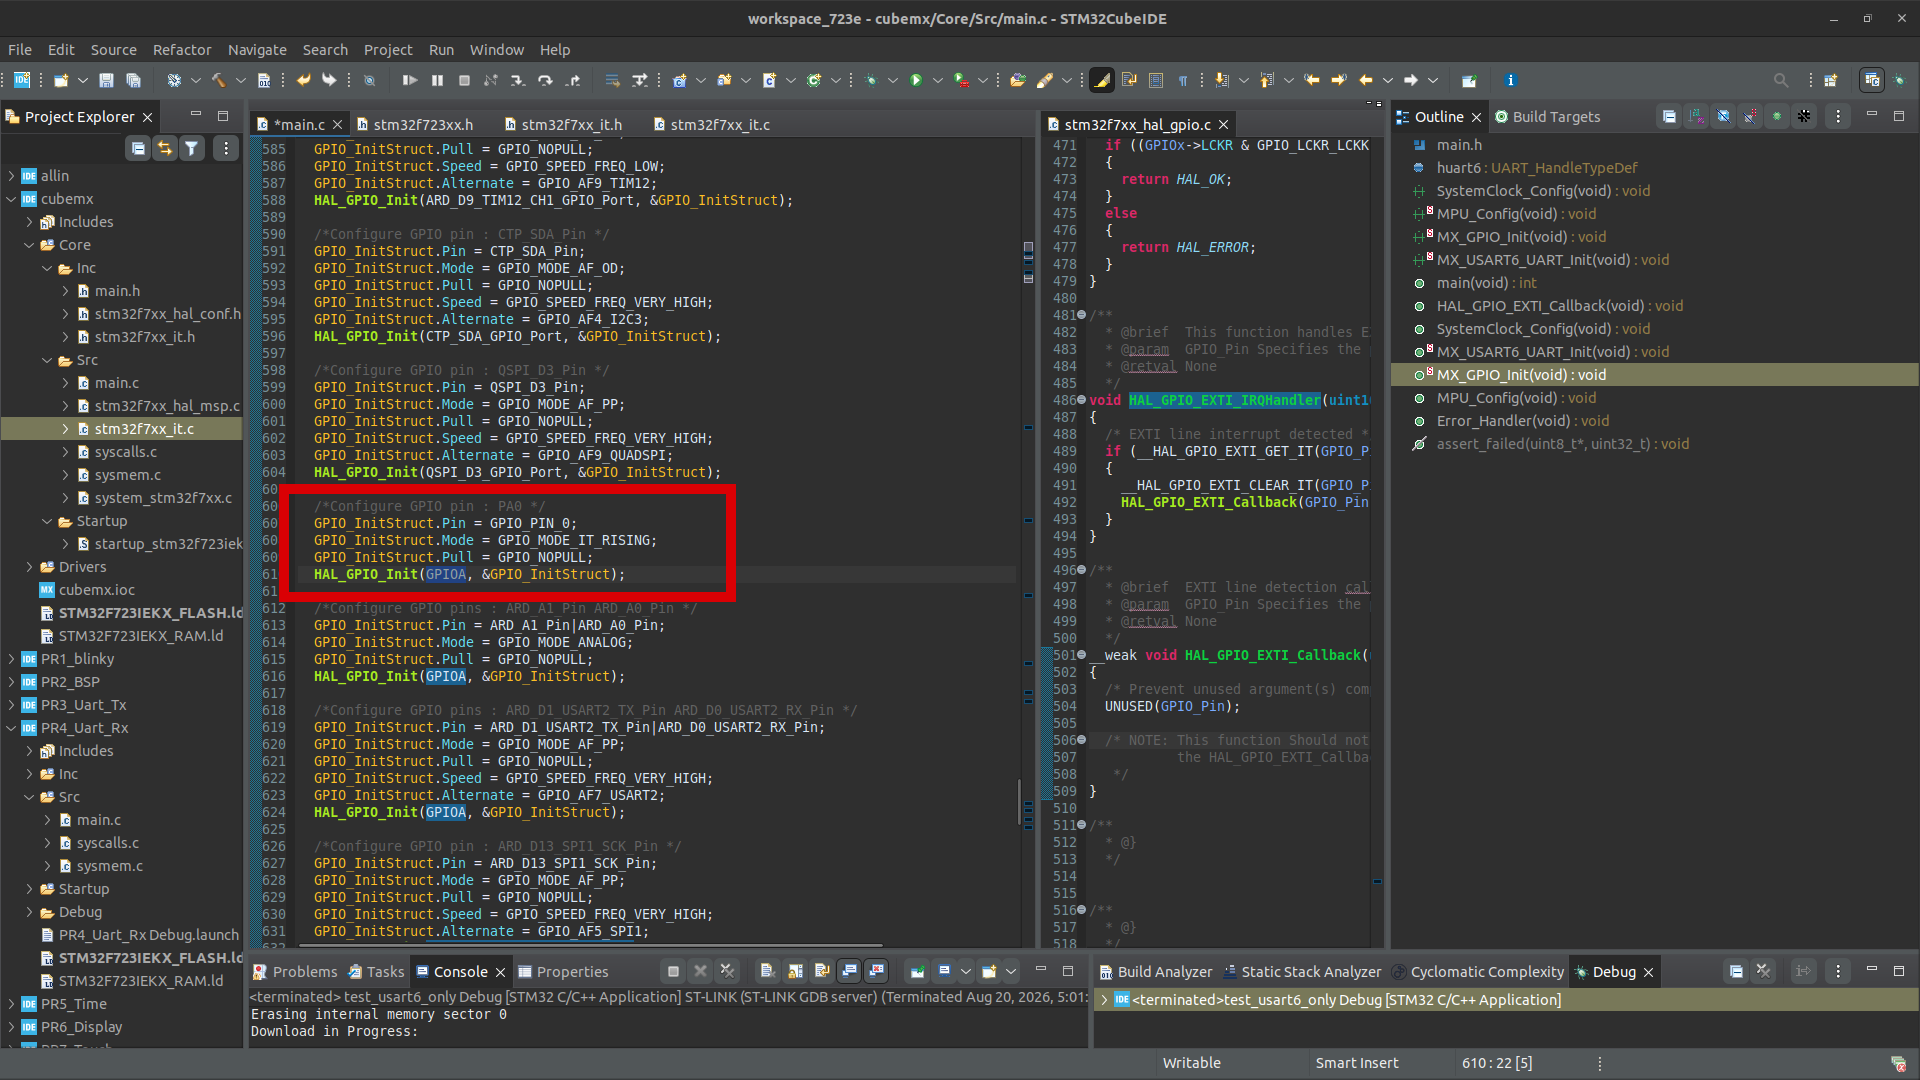
\includegraphics[width=\textwidth]{res/cubeide_07_btnpinsetup.png}
                \caption{Configuración automática del pin para el Botón}
                \label{fig:cubeide_07_btnpinsetup}
            \end{figure}

            Finalmente, nos queda únicamente hacer uso del paquete que se nos ha dado. Haremos un código sencillo donde, cada cierto tiempo, parpadee un LED. Además, al pulsar el botón, enviaremos por la \PER{UART} un texto.

            Si antes esto hubiera supuesto ver la documentación de diferentes periféricos, definir sus estructuras, crear sus funciones auxiliares... ahora podemos directamente hacer uso de las funciones predefinidas en el BSP generado, y nos queda un código muy refinado y corto.

            \begin{lstlisting}
                int main(void)
                {
                    /* MPU Configuration--------------------------------------------------------*/
                    MPU_Config();

                    /* MCU Configuration--------------------------------------------------------*/
                    /* Reset of all peripherals, Initializes the Flash interface and the Systick. */
                    HAL_Init();

                    /* Configure the system clock */
                    SystemClock_Config();

                    /* Initialize all configured peripherals */
                    MX_GPIO_Init();
                    MX_USART6_UART_Init();
                    /* Infinite loop */
                    while (1)
                    {
                        HAL_GPIO_TogglePin(GPIOA, GPIO_PIN_7);
                        HAL_Delay(1000);
                    }
                }

                void HAL_GPIO_EXTI_Callback(uint16_t GPIO_Pin)
                {
                    if (GPIO_Pin == GPIO_PIN_0)
                        HAL_UART_Transmit(&huart6, "Probando\r\n", 10, 1000);
                }
            \end{lstlisting}
            
    
    \subsection{Para hacer más}

        Investiga cómo podrías añadirle aún más funcionalidad al proyecto incluyendo los ficheros de BSP que están en el repositorio \url{https://github.com/STMicroelectronics/STM32Cubef7} (\texttt{Drivers/BSP} y \texttt{Utilities}). Aquí se encuentran drivers de alto nivel para la pantalla o panel táctil, entre otros, así como funciones auxiliares varias.

        \textbf{NOTA:} La adición de estos paquetes es manual, y no se incluyen automáticamente desde STMCubeMX. Tendrás que copiar las carpetas que vayas a utilizar a tu proyecto, y añadir sus rutas a la compilación (\texttt{botón derecho sobre tu proyecto > properties > C/C++ General > Paths and Symbols})

            

\end{document}